\documentclass[a4paper,12pt]{abntex2}
\usepackage{graphicx}
\usepackage{geometry}
\usepackage{hyperref}
\usepackage{fancyhdr}
\usepackage{tcolorbox}
\usepackage{xcolor}
\usepackage{titlesec}
\usepackage{helvet}
\usepackage{array}
\usepackage{amssymb}
\usepackage{booktabs}
\usepackage{longtable}
\usepackage{multirow}
\usepackage{pifont}
\usepackage{colortbl}
\usepackage{makecell}
\usepackage{footmisc}
\usepackage{indentfirst}
\renewcommand{\familydefault}{\sfdefault}

\definecolor{turquoise}{HTML}{00BFB3}
\definecolor{lightblue}{HTML}{D9EEF4}
\definecolor{white}{RGB}{255, 255, 255}
\definecolor{lightgray}{RGB}{200, 200, 200}
\definecolor{footnotecolor}{HTML}{008080}

\makeatletter
\renewcommand\chapter{\@startsection{chapter}{0}{\z@}%
  {-3.5ex \@plus -1ex \@minus -.2ex}%
  {2.3ex \@plus.2ex}%
  {\normalfont\large\bfseries}}
\makeatother


\titleformat{\section}{\normalfont\Large\bfseries}{} {0pt}{}
\arrayrulecolor{white}
\renewcommand{\arraystretch}{1.3}
\newtcolorbox{templatebox}[1][] {colback=turquoise, colframe=turquoise, fontupper=\color{white}\bfseries, boxrule=0mm, arc=0mm, boxsep=4pt, left=2pt, right=2pt, top=2pt, bottom=2pt, width=3cm, halign=center}
\renewcommand{\footnotelayout}{\color{footnotecolor}\small\sffamily}
\geometry{a4paper, margin=1in}
\fancypagestyle{standard}{
    \fancyhf{}
    \fancyfoot[C]{\begin{minipage}[t]{\textwidth} 
    %\raisebox{-0.7\height}{\includegraphics[height=1cm]{GoldStandardLogoFooter.jpg}} 
    %\hspace{0.5cm} \raisebox{-0.5\height}{\textit{Climate Security and Sustainable Development}} 
    \end{minipage}}
    \fancyfoot[R]{\thepage}
    \renewcommand{\headrulewidth}{0pt}
}
\pagestyle{standard}
\fancypagestyle{titlepage}{
    \fancyhf{}
    % \fancyfoot[C]{\begin{minipage}[t]{\textwidth} 
    % \raisebox{-0.7\height}{\includegraphics[height=1cm]{GoldStandardLogoFooter.jpg}} 
    % \hspace{0.5cm} \raisebox{-0.5\height}{\textit{Climate Security and Sustainable Development}} \end{minipage}}
    % \renewcommand{\headrulewidth}{0pt}
}
\begin{document}
\cleardoublepage
%\begin{titlepage}
\thispagestyle{empty}
\vspace*{0pt}
    \begin{center}
        
\includegraphics[width=0.15\textwidth,trim={0.0cm 0.0cm 0.0cm 0.0cm},clip]{templates/LOGOS/IFESlogo.jpg} 
        \hspace{2.0cm}
        
\includegraphics[width=0.25\textwidth,trim={0.0cm 0.5cm 0.0cm 0.0cm},clip]{templates/LOGOS/marca_ufes2_0} 
        \hspace{2.0cm}
        
\includegraphics[width=0.20\textwidth,trim={0.0cm 0.0cm 0.0cm 0.0cm},clip]{templates/LOGOS/Brasao_Governo_1024.png}
    
    
    \vspace{1cm}
    \noindent
    \Large{Análise Tarifária de Unidades Consumidoras com Tarifa Binômia de Energia Elétrica do Governo do Estado do Espírito Santo:}

    \vspace{0.25cm}
    \small{Desenvolvimento de uma Ferramenta Customizada para Acompanhamento dos Contratos e Estudos de Caso}

    \vspace{2.0cm}
    \large{RELATÓRIO DE OTIMIZAÇÃO TARIFÁRIA}

    \textbf{ {{ Unidade }} }

    \vspace{0.15cm}
    
    \small{ {{ Autores }} }
\end{center}  
    \vspace{3cm}

    \arrayrulecolor{lightgray} 
    \noindent

    \begin{table}[!ht]
        \centering
        \setlength{\tabcolsep}{5pt}
        \renewcommand{\arraystretch}{1.3}
        \resizebox{1.0\textwidth}{!}{
        \begin{tabular}{|>{\centering\arraybackslash}p{4cm}|>{\centering\arraybackslash}p{4cm}|>
        {\centering\arraybackslash}p{12cm}|} \hline
        \textbf{Versão} & 
        \textbf{Data} & \textbf{Alterações}\\ \hline
        0 - Emissão inicial& {{ data }} & -\\ \hline
        &  & \\ \hline
        &  & \\ \hline
        &  & \\ \hline
        &  & \\ \hline
        &  & \\ \hline
        &  & \\ \hline
    \end{tabular}
    }
    \end{table} 
    \vfill
    
    \newpage

\chapter{ESCOPO}
O presente relatório apresenta os dados de fornecimento e consumo de energia elétrica da unidade consumidora, obtidos através de suas contas de energia elétrica, além da proposição de otimização tarifária da unidade consumidora e potenciais benefícios financeiros obtidos com a adoção da medida proposta.

\chapter{DADOS DA UNIDADE CONSUMIDORA}

A unidade consumidora analisada é a {{ Unidade }}, localizada na {{ Endereco }}. Possui ramal de entrada em {{ NivelTensao }}, de {{ tensao }} {{ tensaoUnid }}, na área de concessão da distribuidora {{ distribuidora }} cadastrada com o número de instalação {{ instalacao }}.

A edificação  é  um  cliente  {{TipoContrato}}, enquadrado no grupo {{ grupoAtual }}, subgrupo {{ subGrupoAtual }}, classe {{ classe }}. Sua modalidade tarifária atual é a {{ TarifaAtual }} e sua demanda contratada é de {{ demandaAtual }}.

\chapter{HISTÓRICO DE CONSUMO ANALISADO}
Foram  encaminhadas  {{ numContas }}  contas  de  energia  elétrica  consecutivas  da  {{ Unidade }}, 
entre  {{ baseDadosInic }} e {{ baseDadosFinal }}. Após análise dos dados de consumo, optou-se em realizar 
o  estudo  de  otimização  tarifária  com  base  no  intervalo  entre  {{ dadosAnaliseInic }}  e
{{ dadosAnaliseFinal }}.  Além  disso,  a  utilização  de  um  ano  completo  preserva  as  características 
sazonais do perfil de consumo, como pode ser observado na Figura \ref{fig:grafico1}. A Tabela \ref{tab:tabela1} mostra 
os dados mensais de consumo da {{ Unidade }} no período indicado.


\begin{figure}[!ht]
    \centering
    \caption{Histórico da demanda máxima medida}
    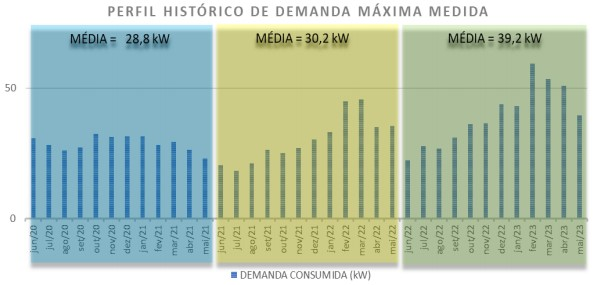
\includegraphics[width=0.85\textwidth]{templates/FIGS/grafico1}
    \label{fig:grafico1}
\end{figure}

\begin{table}[!ht]
    \centering
    \caption{Dados mensais de consumo}
    \label{tab:tabela1}
    \setlength{\tabcolsep}{5pt}
    \renewcommand{\arraystretch}{1.3}
    \rowcolors{2}{white}{lightgray}
    \resizebox{1.0\textwidth}{!}{
    \begin{tabular}{|>{\centering\arraybackslash}p{2cm}|>{\centering\arraybackslash}p{3cm}|>
    {\centering\arraybackslash}p{3cm}|>
    {\centering\arraybackslash}p{3cm}|>
    {\centering\arraybackslash}p{3cm}|>
    {\centering\arraybackslash}p{3cm}|>
    {\centering\arraybackslash}p{3cm}|} \hline
    
    \textbf{Data} & 
    \textbf{Demanda Medida Ponta (KW)} & \textbf{Demanda Medida Fora Ponta (KW)} & \textbf{Energia Ativa de Ponta (KWH)} & 
    \textbf{Energia Ativa de Fora Ponta (KWH)} &
    \textbf{ERE (kWh)} &
    \textbf{Valor Total da Conta de Energia (R\$)} \\\hline
    
    
    \textbf{ {{ row.data }} } & {{ row.demanda_ponta }} & {{ row.demanda_fora_ponta }} & 
    {{ row.energia_ponta }} & {{ row.energia_fora_ponta }} & 
    {{ row.ere }} & {{ row.valor_total }} \\\hline
    
    \multicolumn{6}{|c|}{\textbf{TOTAL}} & \textbf{{ total_energia }} \\\hline

    % mai/23 & 26,17 & 40,49 & 861,93 & 8.862,09 & 0,95 & 7.074,85 \\ \hline
    % abr/23 & 32,32 & 52,10 & 1.093,16 & 11.336,58 & 0,80 & 9.657,80 \\ \hline
    % mar/23 & 32,08 & 54,86 & 1.626,68 & 15.570,34 & 0,06 & 12.653,70 \\ \hline
    % fev/23 & 32,91 & 60,86 & 1.187,33 & 13.253,72 & 0,00 & 11.509,52 \\ \hline
    % jan/23 & 25,93 & 44,28 & 1.133,37 & 11.960,48 & 0,00 & 10.249,06 \\ \hline
    % dez/22 & 27,36 & 44,92 & 1.006,83 & 10.513,06 & 0,00 & 8.347,57 \\ \hline
    % nov/22 & 26,76 & 37,34 & 955,65 & 10.722,27 & 2,45 & 7.637,68 \\ \hline
    % out/22 & 24,31 & 32,14 & 897,78 & 10.616,97 & 0,80 & 7.061,13 \\ \hline
    % set/22 & 21,89 & 31,73 & 804,36 & 7.492,03 & 1,59 & 5.816,13 \\ \hline
    % ago/22 & 21,01 & 27,45 & 856,19 & 7.225,33 & 0,00 & 5.600,62 \\ \hline
    % jul/22 & 19,58 & 28,44 & 830,94 & 7.851,42 & 0,36 & 5.346,39 \\ \hline
    % jun/22 & 18,15 & 22,78 & 778,11 & 6.946,11 & 1,32 & 4.920,74 \\ \hline
    % \multicolumn{6}{|c|}{\textbf{TOTAL} } & \textbf{95.446,12} \\ \hline
    \end{tabular}
    }
    \fonte{Contas de energia elétrica da edificação.}
    \end{table}
    A análise tarifária teve início com a comparação dos valores demandados por mês com o 
    valor contratado de {{ demandaAtual }}. A Figura \ref{fig:grafico2} mostra os valores de demanda medida ponta e fora 
    ponta comparados ao valor contratado junto à concessionária.

    \begin{figure}[!ht]
        \centering
        \caption{Comparação de Demanda Contratada e Medida}
        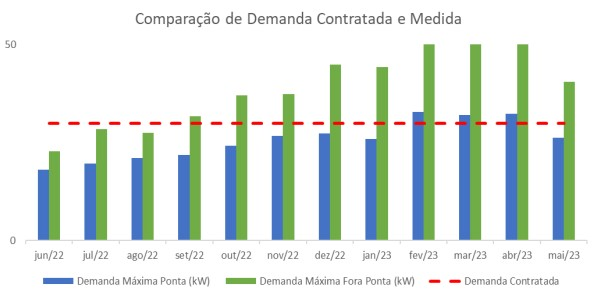
\includegraphics[width=0.85\textwidth]{templates/FIGS/grafico2}
        \label{fig:grafico2}
        \fonte{Contas de energia elétrica da edificação.}
    \end{figure}

Como pode ser visto na Figura \ref{fig:grafico2}, existe ultrapassagem da demanda contratada dentro dos 
meses analisados, pois a demanda máxima medida foi superior em alguns meses  do que a demanda contratada
({{ demandaAtual }}), sendo assim um indicativo que seja viável aumentar  o valor de  demanda  contratada
e,  consequentemente,  obter  uma  economia  monetária  com  a adoção desta medida. 

\chapter{DEMAIS PREMISSAS ADOTADAS}
Além considerar na análise tarifária os últimos 12 meses de consumo como base de dados, 
foram adotadas outras premissas para realizar a análise tarifária:

\begin{itemize}
    \item As  tarifas  de  aplicação  adotadas  nesta  análise  tarifária  são  provenientes  da RESOLUÇÃO HOMOLOGATÓRIA  Nº 3.091, DE 2 DE AGOSTO DE 2022, homologada pela ANEEL (Agência Nacional de Energia Elétrica), ou seja, foram considerados os valores atuais aplicados pela concessionária local;
    \item Como as alíquotas do PIS e COFINS variam mensalmente e não possuem um valor definido  para os  próximos  anos, para  realizar as  análises  foi  considerado um  valor  fixo mensal de alíquota  para esses tributos, cujos valores são definidos com base na média aritmética dos tributos incidentes nos meses adotados (junho/2022 a maio/2023);
    \item A alíquota do ICMS considerada na análise é a mesma registrada nos 12 meses dascontas de energia do cliente (junho/2022 a maio/2023).
    \item Os  valores  e  os  meses  que  incidem  as  bandeiras  tarifárias  serão  os  mesmos registrados nos 12 meses na conta de energia do cliente (junho/2022 a maio/2023)
\end{itemize}

A Tabela \ref{tab:tabela2} apresenta as tarifas aplicadas nesta análise tarifária bem como os valores de 
alíquota de impostos, com base nas premissas adotadas.

\begin{table}[!ht]
\centering
\caption{Resumo das tarifas e alíquotas de impostos adotadas no relatório}
\label{tab:tabela2}
\setlength{\tabcolsep}{5pt}
\renewcommand{\arraystretch}{1.3}
\resizebox{1.0\textwidth}{!}{
\begin{tabular}{|>{\centering\arraybackslash}m{3cm}|>{\centering\arraybackslash}m{2.4cm}|>
{\centering\arraybackslash}m{2.4cm}|>
{\centering\arraybackslash}m{2.4cm}|>
{\centering\arraybackslash}m{2.3cm}|>
{\centering\arraybackslash}m{2.3cm}|>
{\centering\arraybackslash}m{1.5cm}|>
{\centering\arraybackslash}m{1.7cm}|>
{\centering\arraybackslash}m{1.7cm}|>
{\centering\arraybackslash}m{1.7cm}|}
\hline
\textbf{GRUPO\newline MODALIDADE SUBGRUPO} & \textbf{Consumo Ativo de Ponta (R\$/KWh)} & \textbf{Consumo Ativo Fora de Ponta (R\$/KWh)} & \textbf{Demanda Ponta (R\$/kW)} & \textbf{Demanda Fora de Ponta (R\$/kW)} & \textbf{ERE (R\$/KWh)} & \textbf{PIS (\%)} & \textbf{COFINS (\%)} & \textbf{ICMS (\%)} \\ \hline





{\cellcolor{green!30}{{ linha.grupo }}} &

{\cellcolor{blue!30}{{ linha.grupo }}} &

{\cellcolor{red!20}{{ linha.grupo }}} &

{{ linha.grupo }}}

{# Consumo - com ou sem multicolumn #}

\multicolumn{2}{c|}{ {{ linha.consumo_ponta }} } &

{{ linha.consumo_ponta }} & {{ linha.consumo_fora_ponta }} &


{# Demanda - com ou sem multicolumn #}

\multicolumn{2}{c|}{ {{ linha.demanda_ponta }} } &

{{ linha.demanda_ponta }} & {{ linha.demanda_fora }} &


{# Impostos com multirow na primeira linha apenas #}

\multirow{ {{ rowspan }} }{*}{ {{ linha.ere }} } &
\multirow{ {{ rowspan }} }{*}{ {{ linha.pis }} } &
\multirow{ {{ rowspan }} }{*}{ {{ linha.cofins }} } & 
\multirow{ {{ rowspan }} }{*}{ {{ linha.icms }} } \\ 

& & & \\

\cline{1-5}
{# Coloca o \hline apenas na última linha #}

\hline





% \textbf{A VERDE A4} & 1,6628 & 0,39813 & \multicolumn{2}{c|}{30,44} & \multirow{3}{*}{0,27703} & \multirow{3}{*}{1,03916} & \multirow{3}{*}{4,78583} & \multirow{3}{*}{0,00} \\
% \cline{1-5}
% \textbf{A AZUL A4} & 0,55693 & 0,39813 & 45,59 & 30,44 & & & & \\
% \cline{1-5}
% \textbf{BT Optante B3} & \multicolumn{2}{c|}{0,67384} & \multicolumn{2}{c|}{-} & & & & \\
% \hline
\end{tabular}
}
\fonte{Elaborado pelo autor}
\end{table}

\chapter{CUSTO ATUAL COM ENERGIA ELÉTRICA COM BASE NAS PREMISSAS ADOTADAS}
As tarifas de aplicação da {{distribuidora}} são reajustadas anualmente no mês de agosto. Por tal 
motivo,  nas  premissas  adotadas  neste  trabalho  foram  utilizadas  as  tarifas  de  aplicação 
vigentes, com o intuito de que o resultado da economia estimada com o ajuste do contrato 
de energia seja o mais fidedigno possível no futuro. A Tabela \ref{tab:tabela3} mostra os valores mensais 
das  contas  de  energia  da  {{Unidade}}  que  ocorreram,  no  período  {{dadosAnaliseInic}}  a 
{{dadosAnaliseFinal}},  conforme  as  notas  fiscais  das  contas  de  energia  (denominado  “CUSTO 
REALIZADO”) e os valores atualizados considerando as premissas adotadas (denominado “CUSTO ATUALIZADO”).

\begin{table}[!ht]
    \centering
    \caption{Comparação entre os valores de conta realizados e atualizados.}
    \label{tab:tabela3}
    \setlength{\tabcolsep}{5pt}
    \renewcommand{\arraystretch}{1.3}
    \rowcolors{2}{white}{lightgray}
    \resizebox{0.7\textwidth}{!}{
    \begin{tabular}{|>{\centering\arraybackslash}p{4cm}|>{\centering\arraybackslash}p{5cm}|>
    {\centering\arraybackslash}p{5cm}|} \hline
    \textbf{Mês} & 
    \textbf{Custo Realizado (R\$)} & \textbf{Custo Atualizado (R\$)}\\ \hline
    
    
    \textbf{ {{ linha.mes }}} & \textbf{R\$ {{ linha.realizado }}} & \textbf{R\$ {{ linha.atualizado }}} \\
    
    {{ linha.mes }} & R\$ {{ linha.realizado }} & R\$ {{ linha.atualizado }} \\
    
    \hline
    
\end{tabular}
}
\fonte{Elaborado pelo autor}
\end{table} 
Após a consideração das premissas, houve  um aumento  do custo anual nas contas  de 
energia de R\$ {{ ajuste_acrescimo }}, uma variação percentual de aproximadamente {{ ajuste_percentual }} \%. O acréscimo
deve-se ao fato do reajuste das tarifas de aplicação da {{ distribuidora }}, conforme mostrado na 
Tabela \ref{tab:tabela2}. 

\chapter{ANÁLISE DE OTIMIZAÇÃO TARIFÁRIA}
A primeira etapa realizada para proceder a análise de otimização tarifária é verificar quais 
os possíveis enquadramentos tarifários a unidade consumidora pode optar devido às suas 
características.  Após  essa  análise,  verificou-se quais modalidades tarifárias a  edificação  pode  adotar, entre elas a Verde ou Azul do subgrupo {{ subGrupoAtual }} e BT optante (se elegível). As tarifas de aplicação para 
cada enquadramento tarifário supracitado são as previamente apresentadas na Tabela \ref{tab:tabela2}.

Desta forma  foram realizados os procedimentos de otimização de contrat ação de demanda 
das  Tarifas  Horárias  considerando  o  perfil  de  consumo  da  unidade  entre  no  período 
{{ dadosAnaliseInic }}  a  {{ dadosAnaliseFinal }}. Para a {{ TarifaAtual }}, utilizada atualmente, foi verificado 
que é necessário  o aumento  da demanda contratada de  {{ demandaAtual }} para  {{ demandaNova }}. Já na {{ TarifaAnalise }},  as  demandas  contratadas  de  “Ponta”  e  de  “Fora  Ponta”  devem  ser, 
respectivamente,  {{ TarifaAnalisePonta }} e  {{ TarifaAnaliseForaPonta }}.  As tarifas de aplicação para cada enquadramento tarifário 
supracitado são as previamente apresentadas na Tabela \ref{tab:tabela2}.

A  Tabela  \ref{tab:tabela4}  mostra  os  custos  mensais  e  totais  no  período  de  12  meses  para  cada 
modalidade  já  com  a  otimização  de  demanda  (quando  couber)  realizada  conforme  as 
premissas adotadas.

\begin{table}[!ht]
    \centering
    \caption{Comparação entre os valores de conta otimizados}
    \label{tab:tabela4}
    \setlength{\tabcolsep}{5pt}
    \renewcommand{\arraystretch}{1.3}
    \rowcolors{2}{white}{lightblue}
    \resizebox{1.0\textwidth}{!}{

    % \begin{tabular}{|c|c|c|c|}
    % \hline
    % \textbf{DATA} & \cellcolor{green!30}\textbf{A4 Verde Otimizada (R\$)} & \cellcolor{blue!30}\textbf{A4 Azul Otimizada (R\$)} & \cellcolor{red!20}\textbf{BT Optante -- B3 (R\$)} \\
    % \hline
    \begin{tabular}{|c|c|c|c|}
    \hline
    \textbf{DATA} & 
    \cellcolor{green!30}\textbf{A4 Verde Otimizada (R\$)} & 
    \cellcolor{blue!30}\textbf{A4 Azul Otimizada (R\$)} 
    & \cellcolor{red!20}\textbf{BT Optante -- B3 (R\$)}  \\
    \hline
        
    % 
    % 
    % \rowcolor{lightgray}
    % \textbf{ {{ linha.data }} } & \textbf{R\$ {{ linha.verde }} } & \textbf{R\$ {{ linha.azul }} } & \textbf{R\$ {{ linha.bt }} } \\
    % 
    % \textbf{ {{ linha.data }} } & R\$ {{ linha.verde }} & R\$ {{ linha.azul }} & R\$ {{ linha.bt }} \\
    % 
    % \hline
    % 
    
    
    \rowcolor{lightgray}
    \textbf{ {{ linha.data }} } & \textbf{R\$ {{ linha.verde }} } & \textbf{R\$ {{ linha.azul }} } 
    & \textbf{R\$ {{ linha.bt }} } \\
    
    \textbf{ {{ linha.data }} } & R\$ {{ linha.verde }} & R\$ {{ linha.azul }}
    & R\$ {{ linha.bt }} \\
    
    \hline
    
    \end{tabular}
    }
    \fonte{Elaborado pelo autor}
    \end{table}

Após a comparação dos resultados da Tabela \ref{tab:tabela4}, percebe-se que a modalidade tarifária 
mais adequada ao perfil de consumo da unidade consumidora (CONTRATO PROPOSTO) 
com base nas premissas adotadas é a  {{ TarifaNova }}. A Tabela \ref{tab:tabela5} mostra o custo mensal 
das contas de energia, por rubrica, com a adoção da contratação proposta.

\begin{table}[!ht]
    \centering
    \caption{Comparação dos custos mensais considerando o CONTRATO ATUAL e o CONTRATO PROPOSTO.}
    \label{tab:tabela5}
    \setlength{\tabcolsep}{4pt}
    \renewcommand{\arraystretch}{1.3}
    \rowcolors{2}{white}{lightgray}
    \resizebox{1.0\textwidth}{!}{
        \begin{tabular}
            {|>{\centering\arraybackslash}m{2.5cm}|>
            {\centering\arraybackslash}m{3cm}|>
            {\centering\arraybackslash}m{3cm}|>
            {\centering\arraybackslash}m{3cm}|>
            {\centering\arraybackslash}m{3cm}|>
            {\centering\arraybackslash}m{3cm}|>
            {\centering\arraybackslash}m{3cm}|>
            {\centering\arraybackslash}m{3cm}|} \hline
    \textbf{DATA} &
    \textbf{Consumo de energia (R\$)} &
    \textbf{Demanda (R\$)} &
    \textbf{Ultrapassagem (R\$)} &
    \makecell{\textbf{Bandeira e} \\ \textbf{Iluminação} \\ \textbf{Pública (R\$)}} &
    \textbf{ERE (R\$)} &
    \textbf{Impostos (PIS+COFINS) (R\$)} &
    \textbf{TOTAL Conta (R\$)} \\ \hline
    
    {{ linha.data }} & {{ linha.consumo }} & {{ linha.demanda }} & {{ linha.ultrapassagem }} &
    {{ linha.bip }} & {{ linha.ere }} & {{ linha.impostos }} & {{ linha.total }} \\
    \hline
    
    \end{tabular}
    }
    \fonte{Elaborado pelo autor}
    \end{table}

Desta forma, estima-se que o custo anual com as contas de energia após a adequação no 
contrato reduza de R\$ {{ custoContratoAtual }} para R\$ {{ custoContratoNovo }}, ou seja, uma economia monetária de 
aproximadamente R\$ {{ economiaContrato }} por ano, equivalendo a uma redução percentual de {{ economiaPercentual }} \%.
Cabe ressaltar que o fato mais relevante para se obter a economia foi o ajuste na demanda 
contratada.  A Figura \ref{fig:grafico3}  mostra  a  demanda  registrada  mensalmente  e  a  demanda 
contratada após o ajuste de contrato proposto.

\begin{figure}[!ht]
    \centering
    \caption{Comparação de Demanda Contratada e Medida APÓS AJUSTE DE CONTRATO.}
    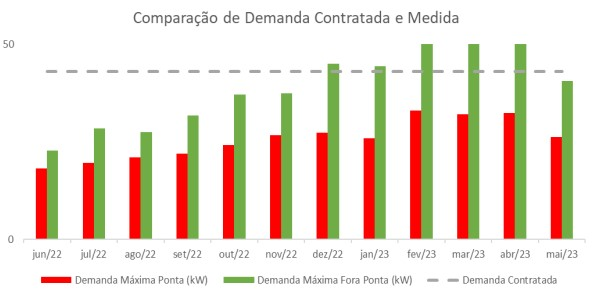
\includegraphics[width=0.85\textwidth]{templates/FIGS/grafico3}
    \label{fig:grafico3}
\end{figure}

\chapter{CONCLUSÕES E AÇÕES PROPOSTAS}
Com base nos estudos executados nas contas de energia elétrica e as premissas adotadas 
nesse relatório, verifica-se que a modalidade tarifária mais adequada ao perfil de consumo 
da unidade consumidora é a {{ TarifaNova }} {{ SubgrupoNovo }}, com demanda contratada de {{ demandaNova }}. Com tal 
ajuste no contrato, estima-se uma economia monetária de aproximadamente  R\$ {{ economiaContrato }}
por ano, que equivale a uma redução percentual de  {{ economiaPercentual }} \%.  A Tabela \ref{tab:tabela6} mostra  de forma 
resumida as recomendações descritas nesse relatório.

\begin{table}[!ht]
    \centering
    \caption{Resumos das ações propostas pelo estudo.}
    \label{tab:tabela6}
    \renewcommand{\arraystretch}{1.3}
    \setlength{\tabcolsep}{6pt}
    \begin{tabular}{|c|c|c|}
    \hline
    \rowcolor[HTML]{EFEFEF}
    \textbf{Contrato} & \textbf{Atual} & \textbf{Proposto} \\
    \hline
    
    
    \rowcolor[HTML]{DDDDDD}
    
    {{ linha.titulo }} & {{ linha.atual }} & {{ linha.proposto }} \\
    \hline
    
    \end{tabular}
    \end{table}

\chapter{DEMAIS RECOMENDAÇÕES}
As  medidas  propostas  geralmente  não  requerem  investimentos  em  aquisição  de 
equipamentos e podem promover uma economia significativa para a unidade analisada. 
Para manutenção desses ganhos, um processo contínuo de monitoramento das faturas de 
energia elétrica deve ser implementado. 
Além  disso, a adoção de boas práticas pode melhorar a utilização da energia elétrica na 
edificação,  por meio  do  seu  uso  racional  e  eficiente.  Seguem  algumas  recomendações 
adicionais para reduzir os custos com aquisição de energia:
\begin{itemize}
    \item  Reduzir o consumo de energia no horário de ponta (entre 18 horas e 21 horas);
    \item  Utilizar equipamentos mais eficientes. Esses equipamentos podem ser identificados 
    por meio do “Selo Procel” que indica os produtos que apresentam os melhores níveis de 
    eficiência energética dentro de cada categoria;
    \item   Apagar lâmpadas e desligar aparelhos de ar-condicionado em ambientes que não 
    estejam sendo utilizados;
    \item  Garantir  a  manutenção  adequada  das  instalações  elétricas  e  dos  equipamentos 
    elétricos e eletrônicos. 
\end{itemize}

\end{document}